\documentclass[a4paper, 11pt]{article}
\usepackage[python]{mypackage}
\usepackage{amsmath}
\usepackage{graphicx}
\usepackage{geometry}
\usepackage{listings}
\geometry{scale=0.8}


\title{
\normalfont \normalsize
\textsc{School of Data and Computer Science, Sun Yat-sen University} \\ [25pt] %textsc small capital letters
\rule{\textwidth}{0.5pt} \\[0.4cm] % Thin top horizontal rule
\huge  E10 Variable Elimination \\ % The assignment title
\rule{\textwidth}{2pt} \\[0.5cm] % Thick bottom horizontal rule
\author{17341015 Hongzheng Chen}
\date{\normalsize\today}
}

\begin{document}
\maketitle
\tableofcontents
\newpage


\section{VE}

The burglary example is described as following:
\begin{figure}[h]
  \centering

  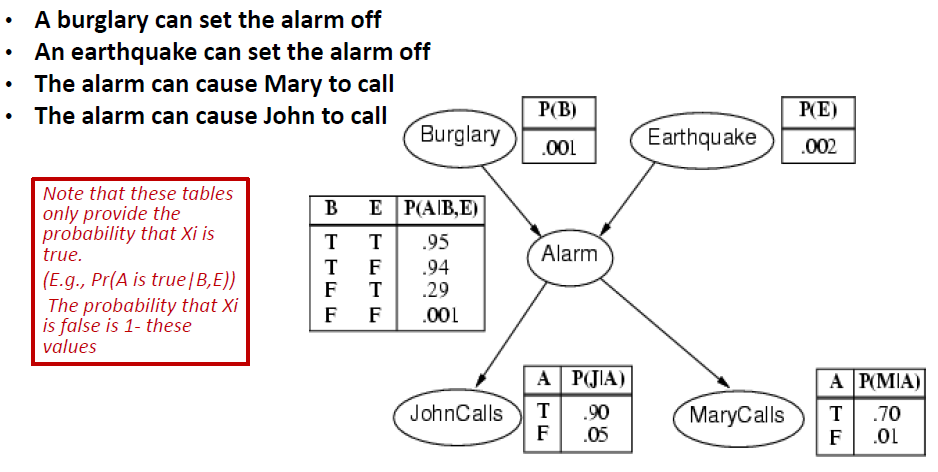
\includegraphics[width=14cm]{fig/burglary}
\end{figure}

\begin{figure}[ht]
\centering
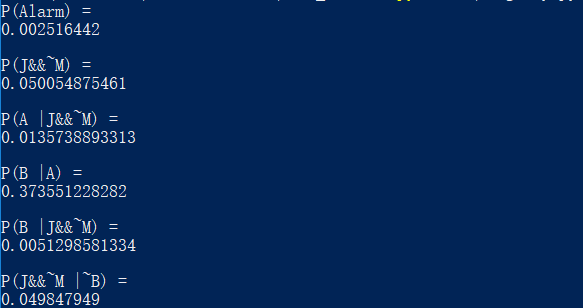
\includegraphics[width=12cm]{fig/burglar_result}
\end{figure}
Here is a VE template for you to solve the burglary example:
\begin{lstlisting}
class VariableElimination:
    @staticmethod
    def inference(factorList, queryVariables,
    orderedListOfHiddenVariables, evidenceList):
        for ev in evidenceList:
            #Your code here
        for var in orderedListOfHiddenVariables:
            #Your code here
        print "RESULT:"
        res = factorList[0]
        for factor in factorList[1:]:
            res = res.multiply(factor)
        total = sum(res.cpt.values())
        res.cpt = {k: v/total for k, v in res.cpt.items()}
        res.printInf()
    @staticmethod
    def printFactors(factorList):
        for factor in factorList:
            factor.printInf()
class Util:
    @staticmethod
    def to_binary(num, len):
        return format(num, '0' + str(len) + 'b')
class Node:
    def __init__(self, name, var_list):
        self.name = name
        self.varList = var_list
        self.cpt = {}
    def setCpt(self, cpt):
        self.cpt = cpt
    def printInf(self):
        print "Name = " + self.name
        print " vars " + str(self.varList)
        for key in self.cpt:
            print "   key: " + key + " val : " + str(self.cpt[key])
        print ""
    def multiply(self, factor):
        """function that multiplies with another factor"""
        #Your code here
        new_node = Node("f" + str(newList), newList)
        new_node.setCpt(new_cpt)
        return new_node
    def sumout(self, variable):
        """function that sums out a variable given a factor"""
        #Your code here
        new_node = Node("f" + str(new_var_list), new_var_list)
        new_node.setCpt(new_cpt)
        return new_node
    def restrict(self, variable, value):
        """function that restricts a variable to some value
        in a given factor"""
        #Your code here
        new_node = Node("f" + str(new_var_list), new_var_list)
        new_node.setCpt(new_cpt)
        return new_node
# create nodes for Bayes Net
B = Node("B", ["B"])
E = Node("E", ["E"])
A = Node("A", ["A", "B","E"])
J = Node("J", ["J", "A"])
M = Node("M", ["M", "A"])

# Generate cpt for each node
B.setCpt({'0': 0.999, '1': 0.001})
E.setCpt({'0': 0.998, '1': 0.002})
A.setCpt({'111': 0.95, '011': 0.05, '110':0.94,'010':0.06,
'101':0.29,'001':0.71,'100':0.001,'000':0.999})
J.setCpt({'11': 0.9, '01': 0.1, '10': 0.05, '00': 0.95})
M.setCpt({'11': 0.7, '01': 0.3, '10': 0.01, '00': 0.99})

print "P(A) **********************"
VariableElimination.inference([B,E,A,J,M], ['A'], ['B', 'E', 'J','M'], {})

print "P(B | J~M) **********************"
VariableElimination.inference([B,E,A,J,M], ['B'], ['E','A'], {'J':1,'M':0})
\end{lstlisting}

\section{Task}
\begin{itemize}
\item You should implement 4 functions: \texttt{inference}, \texttt{multiply}, \texttt{sumout} and \texttt{restrict}. You can turn to Figure \ref{Fig:ve_product} and Figure \ref{Fig:sumout_restrict} for help.
\item Please hand in a file named \textsf{E10\_YourNumber.pdf}, and send it to \textsf{ai\_201901@foxmail.com}
\end{itemize}

\begin{figure}[ht]{}
\centering
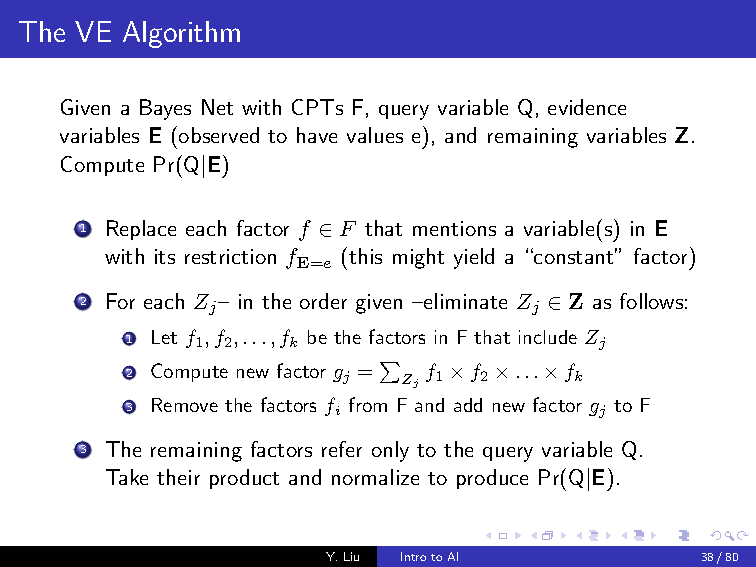
\includegraphics[width=7.5cm]{fig/ve}
\qquad
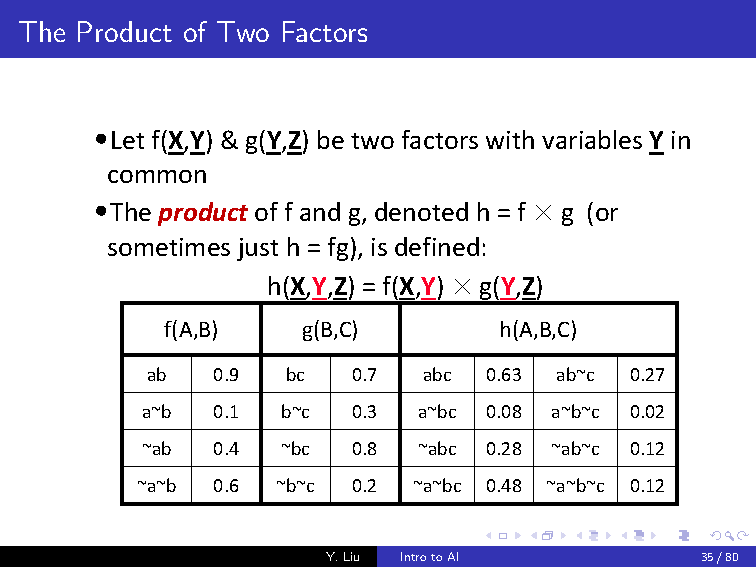
\includegraphics[width=7.5cm]{fig/product}
\caption{VE and Product}
\label{Fig:ve_product}
\end{figure}


\begin{figure}[ht]
\centering
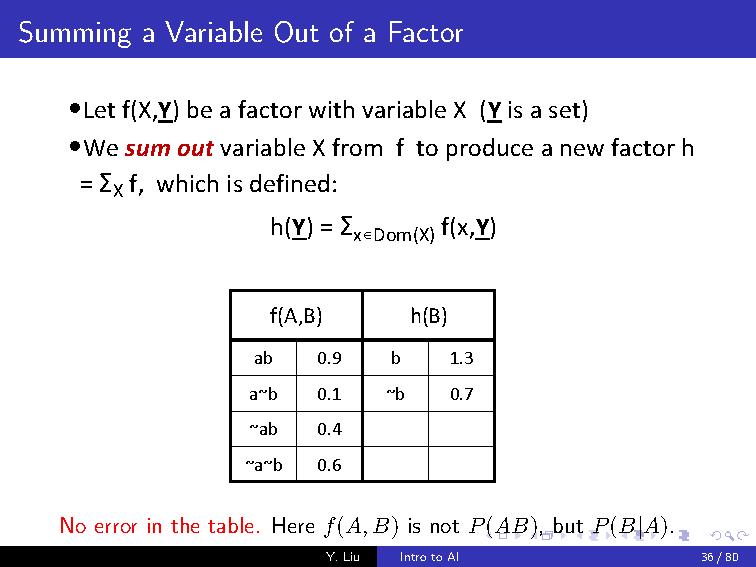
\includegraphics[width=7.5cm]{fig/sumout}
\qquad
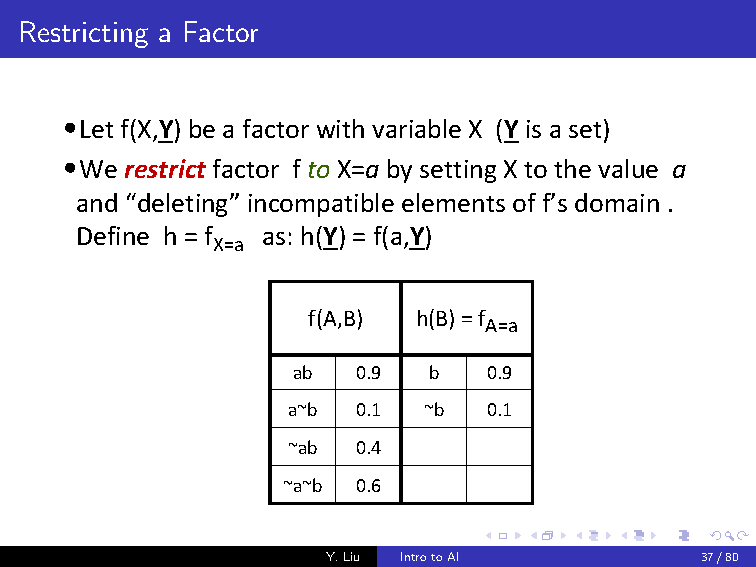
\includegraphics[width=7.5cm]{fig/restrict}
\caption{Sumout and Restrict}
\label{Fig:sumout_restrict}
\end{figure}

\section{Codes and Results}
Codes are listed below.
Notice \textcolor{red}{Python 3} is used!
\begin{lstlisting}
class VariableElimination:
    @staticmethod
    def inference(factorList, queryVariables, orderedListOfHiddenVariables, evidenceList):
        for ev in evidenceList:
            for i,node in enumerate(factorList):
                if ev in node.varList:
                    factorList[i] = node.restrict(ev,evidenceList[ev])
        for var in orderedListOfHiddenVariables:
            # for node in factorList:
            #     print(node.name,end=" ")
            # print()
            newFactorList = []
            for node in factorList:
                if var in node.varList:
                    newFactorList.append(node)
            res = newFactorList[0]
            factorList.remove(res)
            for factor in newFactorList[1:]:
                res = res.multiply(factor)
                factorList.remove(factor)
            res = res.sumout(var)
            factorList.append(res)
        print("RESULT:")
        res = factorList[0]
        for factor in factorList[1:]:
            res = res.multiply(factor)
        total = sum(res.cpt.values())
        res.cpt = {k: v/total for k, v in res.cpt.items()}
        res.printInf()

    @staticmethod
    def printFactors(factorList):
        for factor in factorList:
            factor.printInf()

def get_new_cpt_var(num):
    if num == 0: # be careful!
        return [""]
    cpt_var = []
    format_spec = "{0:0" + str(num) + "b}"
    for i in range(2**num):
        cpt_var.append(format_spec.format(i))
    return cpt_var

class Node:
    def __init__(self, name, var_list):
        self.name = name
        # the first var is itself, others are dependency
        self.varList = var_list
        self.cpt = {}

    def setCpt(self, cpt):
        self.cpt = cpt

    def printInf(self):
        print("Name = " + self.name)
        print(" vars " + str(self.varList))
        for key in self.cpt:
            print("   key: " + key + " val : " + str(self.cpt[key]))
        print()

    def multiply(self, factor):
        """function that multiplies with another factor"""
        var_list_1 = self.varList.copy()
        var_list_2 = factor.varList.copy()
        new_var_list = list(set(var_list_1 + var_list_2)) # take a union
        new_cpt = {}
        cpt_var = get_new_cpt_var(len(new_var_list))
        for var in cpt_var:
            var_dict = {}
            for i,v in enumerate(new_var_list):
                var_dict[v] = var[i]
            item = ""
            for var1 in self.varList:
                item += var_dict[var1]
            f1 = self.cpt[item]
            item = ""
            for var2 in factor.varList:
                item += var_dict[var2]
            f2 = factor.cpt[item]
            new_cpt[var] = f1 * f2
        new_node = Node("f" + str(new_var_list), new_var_list)
        new_node.setCpt(new_cpt)
        # print("{} multiply {} -> {}".format(self.name,factor.name,new_node.name))
        return new_node

    def sumout(self, variable):
        """function that sums out a variable given a factor"""
        index = self.varList.index(variable)
        new_var_list = self.varList.copy()
        new_var_list.remove(variable)
        cpt_var = get_new_cpt_var(len(new_var_list))
        new_cpt = {}
        for var in cpt_var:
            sumup = 0
            for curr in ["0","1"]:
                origin_var = var[:index] + curr + var[index:]
                sumup += self.cpt[origin_var]
            new_cpt[var] = sumup
        new_node = Node("f" + str(new_var_list), new_var_list)
        new_node.setCpt(new_cpt)
        # print("{} sumout {} -> {}".format(self.name,variable,new_node.name))
        return new_node

    def restrict(self, variable, value):
        """function that restricts a variable to some value
        in a given factor"""
        index = self.varList.index(variable)
        new_var_list = self.varList.copy()
        new_var_list.remove(variable)
        cpt_var = get_new_cpt_var(len(new_var_list))
        new_cpt = {}
        for var in cpt_var:
            origin_var = var[:index] + str(value) + var[index:]
            new_cpt[var] = self.cpt[origin_var]
        new_node = Node("f" + str(new_var_list), new_var_list)
        new_node.setCpt(new_cpt)
        # print("{} restricts {} to {} -> {}".format(self.name,variable,value,new_node.name))
        return new_node

# create nodes for Bayes Net
B = Node("B", ["B"])
E = Node("E", ["E"])
A = Node("A", ["A", "B", "E"])
J = Node("J", ["J", "A"])
M = Node("M", ["M", "A"])

# Generate cpt for each node
B.setCpt({'0': 0.999, '1': 0.001})
E.setCpt({'0': 0.998, '1': 0.002})
A.setCpt({'111': 0.95, '011': 0.05, '110':0.94,'010':0.06, '101':0.29, '001':0.71, '100':0.001, '000':0.999})
J.setCpt({'11': 0.9, '01': 0.1, '10': 0.05, '00': 0.95})
M.setCpt({'11': 0.7, '01': 0.3, '10': 0.01, '00': 0.99})

print("P(A) **********************")
VariableElimination.inference([B,E,A,J,M], ['A'], ['B','E','J','M'], {})

print("P(J ~M) **********************")
VariableElimination.inference([B,E,A,J,M], ['J','M'], ['B','E','A'], {})

print("P(A | J~M) **********************")
VariableElimination.inference([B,E,A,J,M], ['A'], ['E','B'], {'J':1,'M':0})

print("P(B | A) **********************")
VariableElimination.inference([B,E,A,J,M], ['B'], ['J','M','E'], {'A':1})

print("P(B | J~M) **********************")
VariableElimination.inference([B,E,A,J,M], ['B'], ['E','A'], {'J':1,'M':0})

print("P(J~M | ~B) **********************")
VariableElimination.inference([B,E,A,J,M], ['J','M'], ['E','A'], {'B':0})
\end{lstlisting}

\begin{figure}[H]
\centering
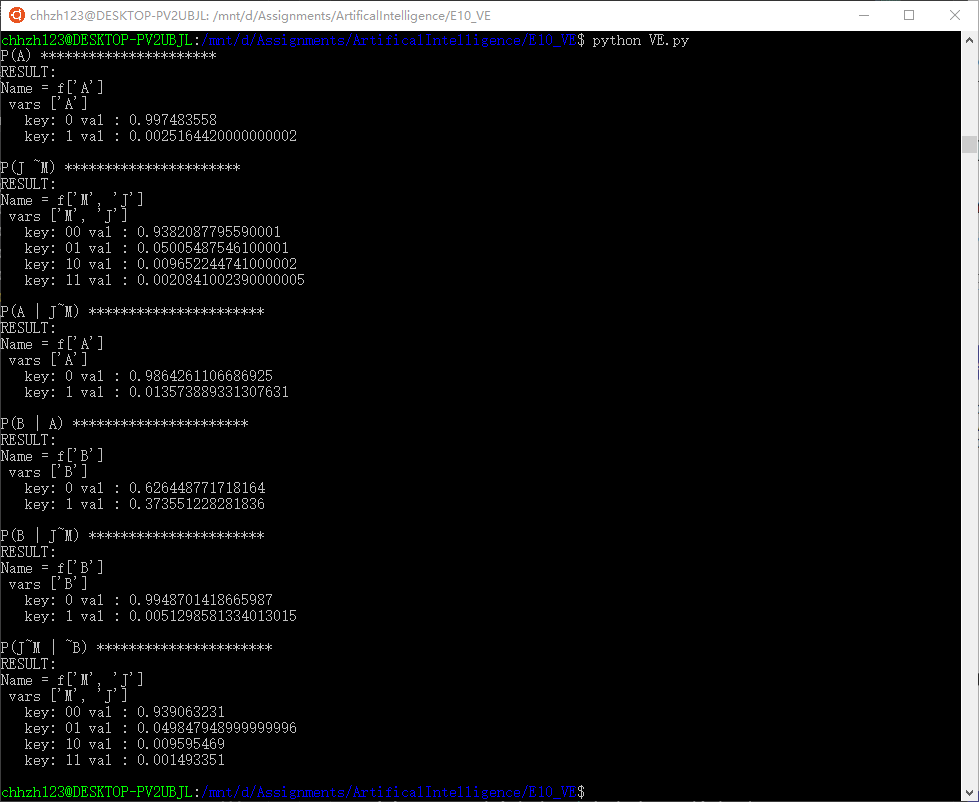
\includegraphics[width=\linewidth]{fig/results.png}
\end{figure}

\end{document}